\begin{ujnbody}
% 以下为正文主体,把点引线以下的文字替换成你的就好
% ·································································································
    \section{功能测试(节标题section)}
    \subsection{文字与段落(子节标题subsection)}
    这是文字。
    \subsubsection{段落(子小节标题subsubsection)}
    这是段落。这是段落。这是段落。这是段落。这是段落。这是段落。这是段落。这是段落。这是段落。这是段落。这是段落。这是段落。这是段落。这是段落。这是段落。这是段落。这是段落。这是段落。这是段落。这是段落。

    这是另一个段落。这是另一个段落。这是另一个段落。这是另一个段落。这是另一个段落。这是另一个段落。这是另一个段落。这是另一个段落。这是另一个段落。这是另一个段落。这是另一个段落。这是另一个段落。这是另一个段落。
    \subsection{数学公式}
    \subsubsection{行内公式}
    这是简单的行内公式:$x^2+y^2=z^2$,这是复杂的行内公式:$\sum_{i=1}^n a_i=0$。
    \subsubsection{行间公式}
    (1)线性代数:
    \begin{equation}
        \begin{split}
            \mathbf{A}^{-1} &= \frac{1}{\det(\mathbf{A})}\mathbf{A}^* \\
            \mathbf{A}^* &= \begin{bmatrix}
                \mathbf{A}_{11}^* & \mathbf{A}_{12}^* & \cdots & \mathbf{A}_{1n}^* \\
                \mathbf{A}_{21}^* & \mathbf{A}_{22}^* & \cdots & \mathbf{A}_{2n}^* \\
                \vdots & \vdots & \ddots & \vdots \\
                \mathbf{A}_{m1}^* & \mathbf{A}_{m2}^* & \cdots & \mathbf{A}_{mn}^*
            \end{bmatrix} \\
        \end{split}
    \end{equation}

    (2)微积分:
    \begin{equation}
        \begin{split}
            \frac{d}{dx}f(x) &= \lim_{h \to 0}\frac{f(x+h)-f(x)}{h} \\
            \frac{d^2}{dx^2}f(x) &= \lim_{h \to 0}\frac{f(x+h)-2f(x)+f(x-h)}{h^2} \\
            \frac{d^n}{dx^n}f(x) &= \lim_{h \to 0}\frac{f(x+h)-f(x)-\cdots-f(x-(n-1)h)}{h^n}
        \end{split}
        \label{eq:1}
    \end{equation}

    (3)概率论与数理统计:
    \begin{equation}
        \begin{split}
            P(A) &= \frac{\text{事件A发生的次数}}{\text{总次数}} \\
            P(A \mid B) &= \frac{P(A \cap B)}{P(B)} \\
            P(A \cap B) &= P(A)P(B \mid A) \\
            P(A \cup B) &= P(A) + P(B) - P(A \cap B)
        \end{split}
    \end{equation}

    \begin{equation}
        \begin{split}
            E(X) &= \sum_{i=1}^n x_iP(X=x_i) \\
            E(XY) &= \sum_{i=1}^n \sum_{j=1}^n x_iy_jP(X=x_i,Y=y_j) \\
            E(X \mid Y) &= \sum_{i=1}^n x_iP(X=x_i \mid Y=y) \\
            E(X \mid Y=y) &= \sum_{i=1}^n x_iP(X=x_i,Y=y) \\
            E(X \mid Y=y_1,y_2,\cdots,y_k) &= \sum_{i=1}^n x_iP(X=x_i,Y=y_1,Y=y_2,\cdots,Y=y_k)
        \end{split}
    \end{equation}

    (4)数学分析:

    \begin{equation}
        \begin{split}
            \lim_{x \to a}f(x) &= L \\
            \lim_{x \to a^+}f(x) &= L \\
            \lim_{x \to a^-}f(x) &= L \\
            \lim_{x \to a^+}f(x) &= \lim_{x \to a^-}f(x) \\
            \lim_{x \to a^+}f(x) &= \lim_{x \to a^-}f(x) = L
        \end{split}
    \end{equation}

    (5)离散数学:
    \begin{equation}
        \begin{split}
            \binom{n}{k} &= \frac{n!}{k!(n-k)!} \\
            \binom{n}{0} &= \binom{n}{n} = 1 \\
            \binom{n}{1} &= \binom{n}{n-1} = n \\
            \binom{n}{2} &= \binom{n}{n-2} = \frac{n(n-1)}{2}
        \end{split}
    \end{equation}

    (6)复变函数:
    \begin{equation}
        \begin{split}
            \lim_{z \to \infty}f(z) &= L \\
            \lim_{z \to \infty}f(z) &= \lim_{z \to -\infty}f(z) \\
            \lim_{z \to \infty}f(z) &= \lim_{z \to -\infty}f(z) = L \\
            \lim_{z \to \infty}f(z) &= \lim_{z \to -\infty}f(z) \neq L
        \end{split}
    \end{equation}
    \subsection{代码块与图表}
    \subsubsection{代码块}
    \begin{lstlisting}[language=C]
        #include <stdio.h>
        /* hello,world */
        int main(){
            printf("Hello, World! \n"); 
            return 0;
        }
    \end{lstlisting}
    \subsubsection{图片}
    \begin{figure}[htbp]
        \centering
        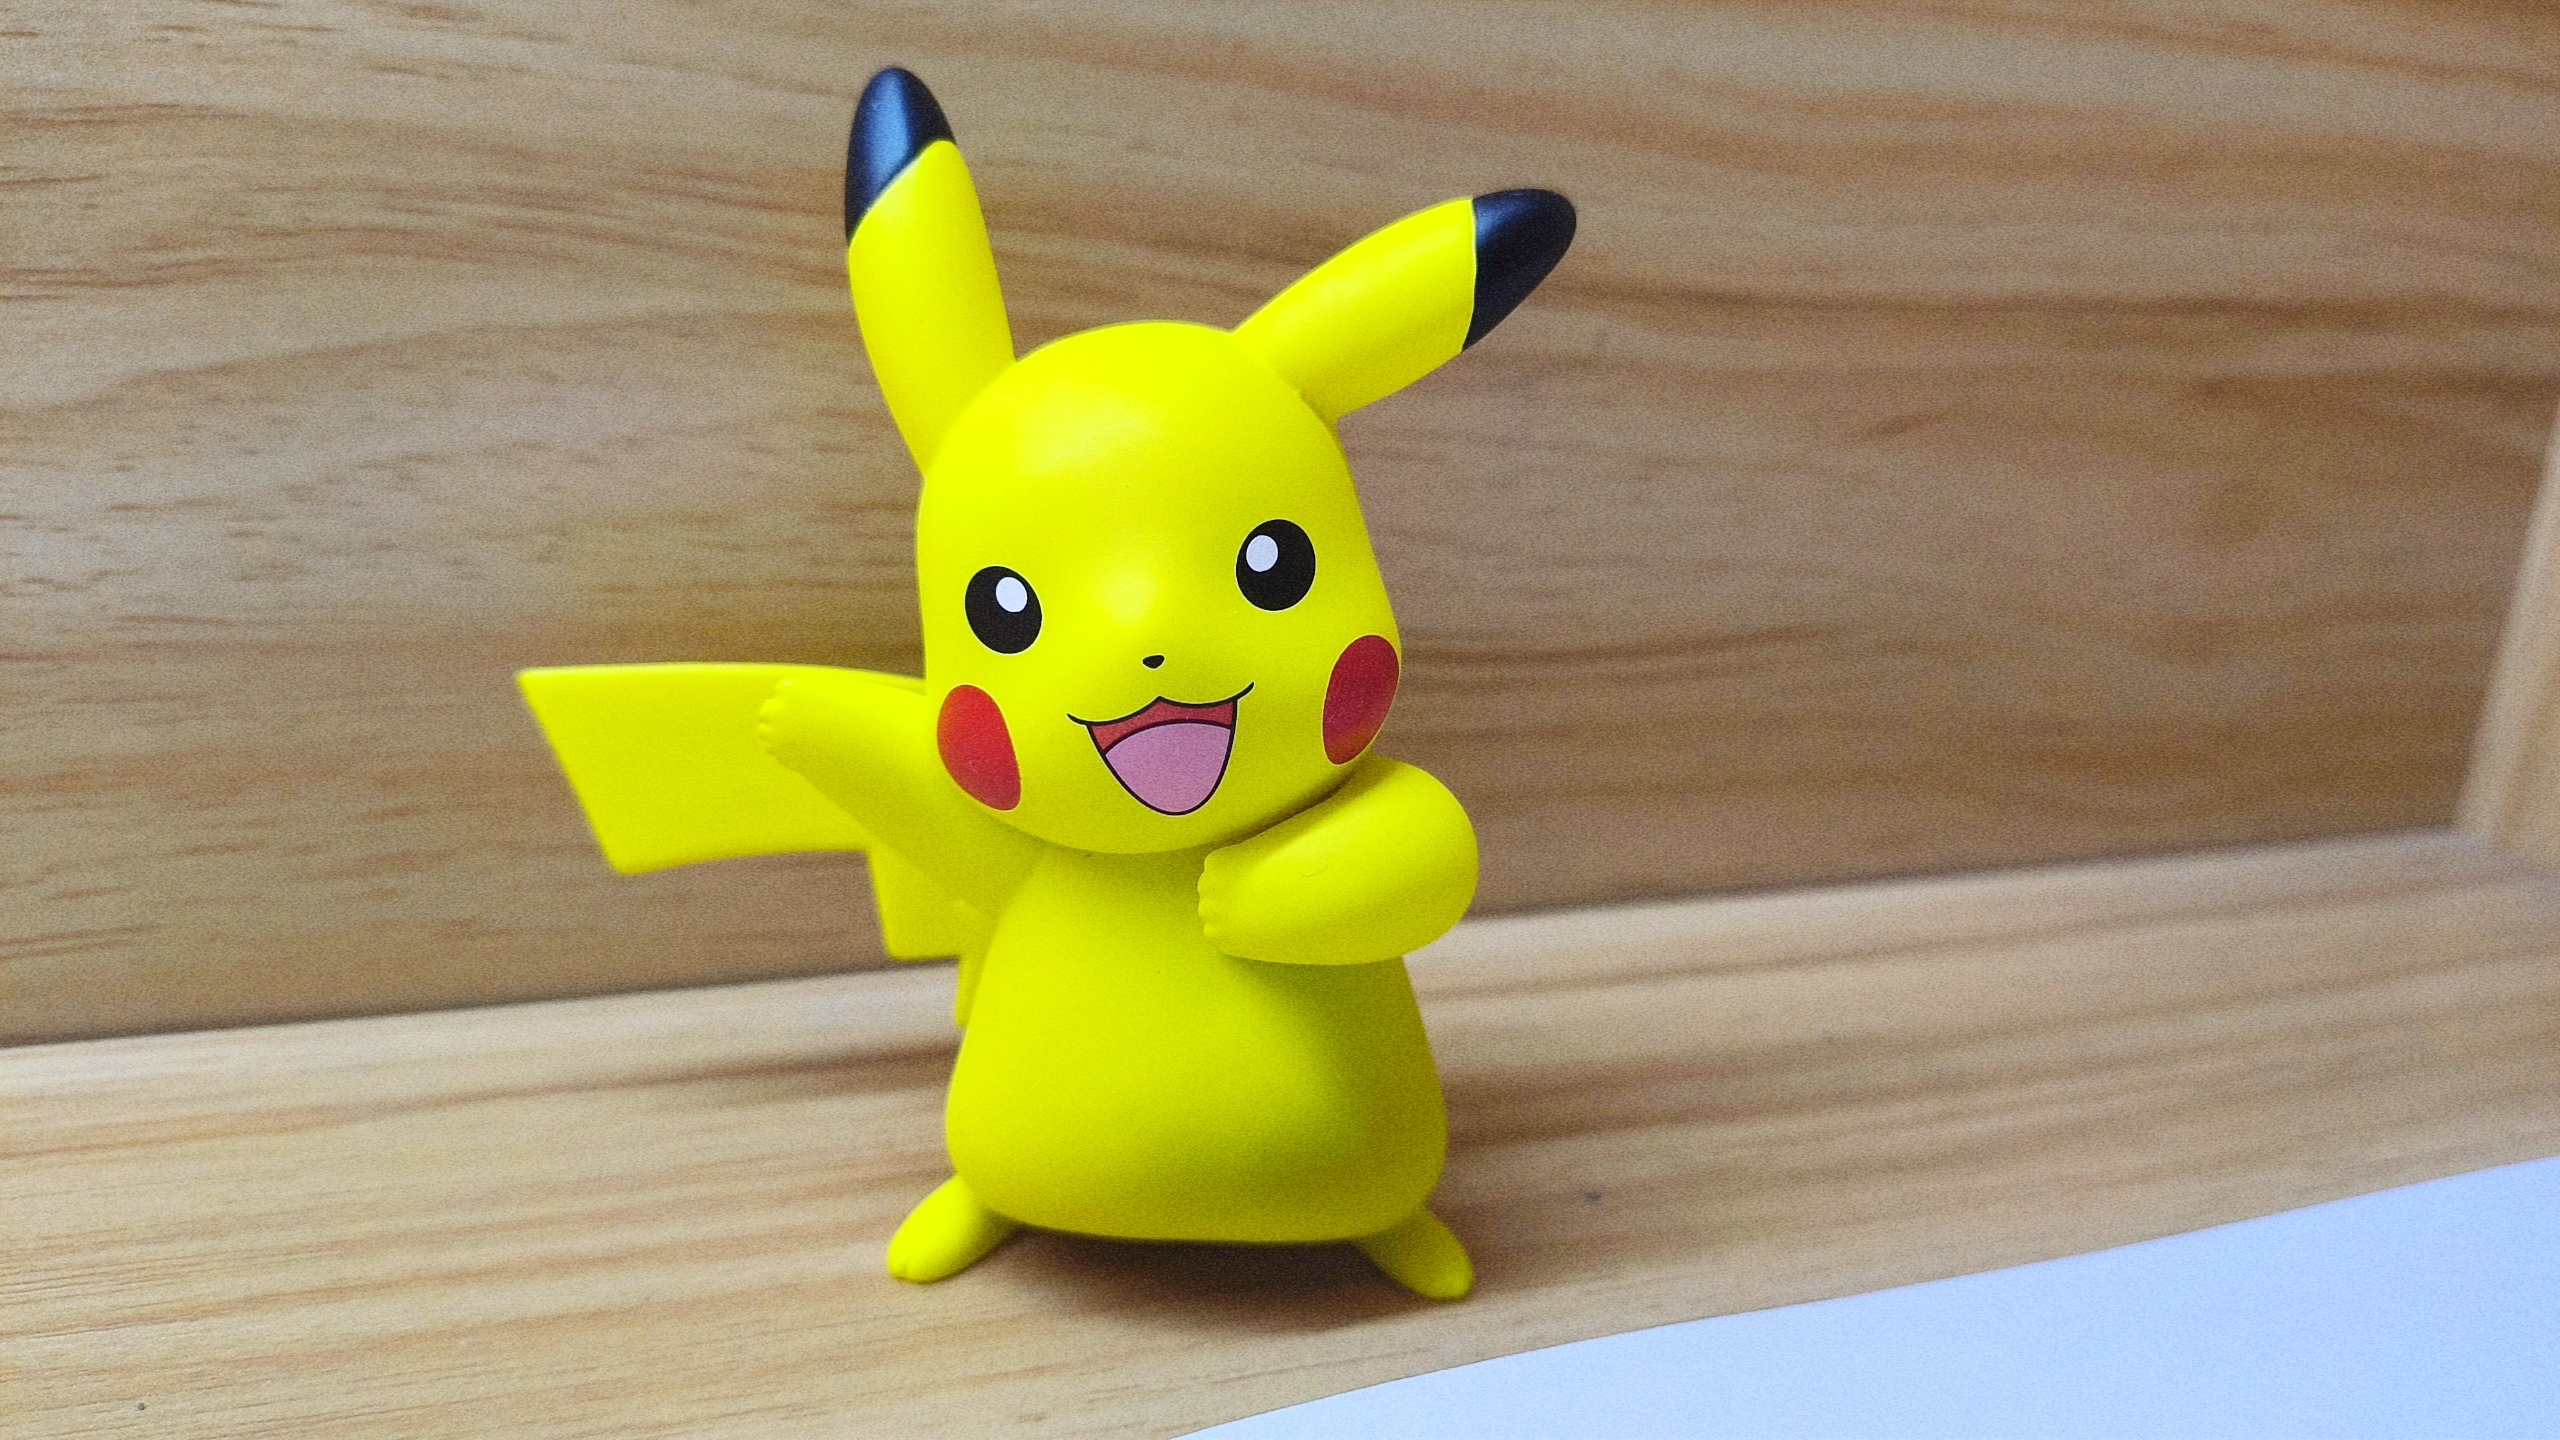
\includegraphics[scale=0.1]{figures/pikachu.jpg}
        \caption{这是图片}
        \label{fig:1}
    \end{figure}
    \subsubsection{表格}
    \begin{table}[!htbp]
        \centering
        \caption{这是表格}
        \begin{tabular}{cccccc}
            \toprule
            序号 & 姓名 & 性别 & 年龄 & 身高/cm & 体重/kg \\
            \midrule
            1 & 张三 & M & 16 & 163 & 50 \\
            2 & 王红 & F & 15 & 159 & 47 \\
            3 & 李二 & M & 17 & 165 & 52 \\
            \bottomrule
        \end{tabular}
        \label{tab:1}
    \end{table}
    \subsection{交叉引用}\label{sec:1}
    \subsubsection{参考文献引用}\label{sec:2}
    首先引用一下大名鼎鼎的香农信息论\cite{shannon1948mathematical},所以哪能少得了图灵\cite{turing2009computing},因为看过《美丽心灵》就还有纳什\cite{nash1996non}。
    \subsubsection{图表引用}
    图片\ref{fig:1}和表格\ref{tab:1}的交叉引用。
    \subsubsection{章节引用}
    章节\ref{sec:1}和章节\ref{sec:2}的交叉引用。
    \subsubsection{公式引用}
    公式\ref{eq:1}的交叉引用。
    \section{功能测试(节标题section)}
    \subsection{文字与段落(子节标题subsection)}
    这是文字。
    \subsubsection{段落(子小节标题subsubsection)}
    这是段落。这是段落。这是段落。这是段落。这是段落。这是段落。这是段落。这是段落。这是段落。这是段落。这是段落。这是段落。这是段落。这是段落。这是段落。这是段落。这是段落。这是段落。这是段落。这是段落。

    这是另一个段落。这是另一个段落。这是另一个段落。这是另一个段落。这是另一个段落。这是另一个段落。这是另一个段落。这是另一个段落。这是另一个段落。这是另一个段落。这是另一个段落。这是另一个段落。这是另一个段落。
    \subsection{数学公式}
    \subsubsection{行内公式}
    这是简单的行内公式:$x^2+y^2=z^2$,这是复杂的行内公式:$\sum_{i=1}^n a_i=0$。
    \subsubsection{行间公式}
    (1)线性代数:
    \begin{equation}
        \begin{split}
            \mathbf{A}^{-1} &= \frac{1}{\det(\mathbf{A})}\mathbf{A}^* \\
            \mathbf{A}^* &= \begin{bmatrix}
                \mathbf{A}_{11}^* & \mathbf{A}_{12}^* & \cdots & \mathbf{A}_{1n}^* \\
                \mathbf{A}_{21}^* & \mathbf{A}_{22}^* & \cdots & \mathbf{A}_{2n}^* \\
                \vdots & \vdots & \ddots & \vdots \\
                \mathbf{A}_{m1}^* & \mathbf{A}_{m2}^* & \cdots & \mathbf{A}_{mn}^*
            \end{bmatrix} \\
        \end{split}
    \end{equation}

    (2)微积分:
    \begin{equation}
        \begin{split}
            \frac{d}{dx}f(x) &= \lim_{h \to 0}\frac{f(x+h)-f(x)}{h} \\
            \frac{d^2}{dx^2}f(x) &= \lim_{h \to 0}\frac{f(x+h)-2f(x)+f(x-h)}{h^2} \\
            \frac{d^n}{dx^n}f(x) &= \lim_{h \to 0}\frac{f(x+h)-f(x)-\cdots-f(x-(n-1)h)}{h^n}
        \end{split}
        \label{eq:2}
    \end{equation}

    (3)概率论与数理统计:
    \begin{equation}
        \begin{split}
            P(A) &= \frac{\text{事件A发生的次数}}{\text{总次数}} \\
            P(A \mid B) &= \frac{P(A \cap B)}{P(B)} \\
            P(A \cap B) &= P(A)P(B \mid A) \\
            P(A \cup B) &= P(A) + P(B) - P(A \cap B)
        \end{split}
    \end{equation}

    \begin{equation}
        \begin{split}
            E(X) &= \sum_{i=1}^n x_iP(X=x_i) \\
            E(XY) &= \sum_{i=1}^n \sum_{j=1}^n x_iy_jP(X=x_i,Y=y_j) \\
            E(X \mid Y) &= \sum_{i=1}^n x_iP(X=x_i \mid Y=y) \\
            E(X \mid Y=y) &= \sum_{i=1}^n x_iP(X=x_i,Y=y) \\
            E(X \mid Y=y_1,y_2,\cdots,y_k) &= \sum_{i=1}^n x_iP(X=x_i,Y=y_1,Y=y_2,\cdots,Y=y_k)
        \end{split}
    \end{equation}

    (4)数学分析:

    \begin{equation}
        \begin{split}
            \lim_{x \to a}f(x) &= L \\
            \lim_{x \to a^+}f(x) &= L \\
            \lim_{x \to a^-}f(x) &= L \\
            \lim_{x \to a^+}f(x) &= \lim_{x \to a^-}f(x) \\
            \lim_{x \to a^+}f(x) &= \lim_{x \to a^-}f(x) = L
        \end{split}
    \end{equation}

    (5)离散数学:
    \begin{equation}
        \begin{split}
            \binom{n}{k} &= \frac{n!}{k!(n-k)!} \\
            \binom{n}{0} &= \binom{n}{n} = 1 \\
            \binom{n}{1} &= \binom{n}{n-1} = n \\
            \binom{n}{2} &= \binom{n}{n-2} = \frac{n(n-1)}{2}
        \end{split}
    \end{equation}

    (6)复变函数:
    \begin{equation}
        \begin{split}
            \lim_{z \to \infty}f(z) &= L \\
            \lim_{z \to \infty}f(z) &= \lim_{z \to -\infty}f(z) \\
            \lim_{z \to \infty}f(z) &= \lim_{z \to -\infty}f(z) = L \\
            \lim_{z \to \infty}f(z) &= \lim_{z \to -\infty}f(z) \neq L
        \end{split}
    \end{equation}
    \subsection{代码块与图表}
    \subsubsection{代码块}
    \begin{lstlisting}[language=C]
        #include <stdio.h>
        /* hello,world */
        int main(){
            printf("Hello, World! \n"); 
            return 0;
        }
    \end{lstlisting}
    \subsubsection{图片}
    \begin{figure}[htbp]
        \centering
        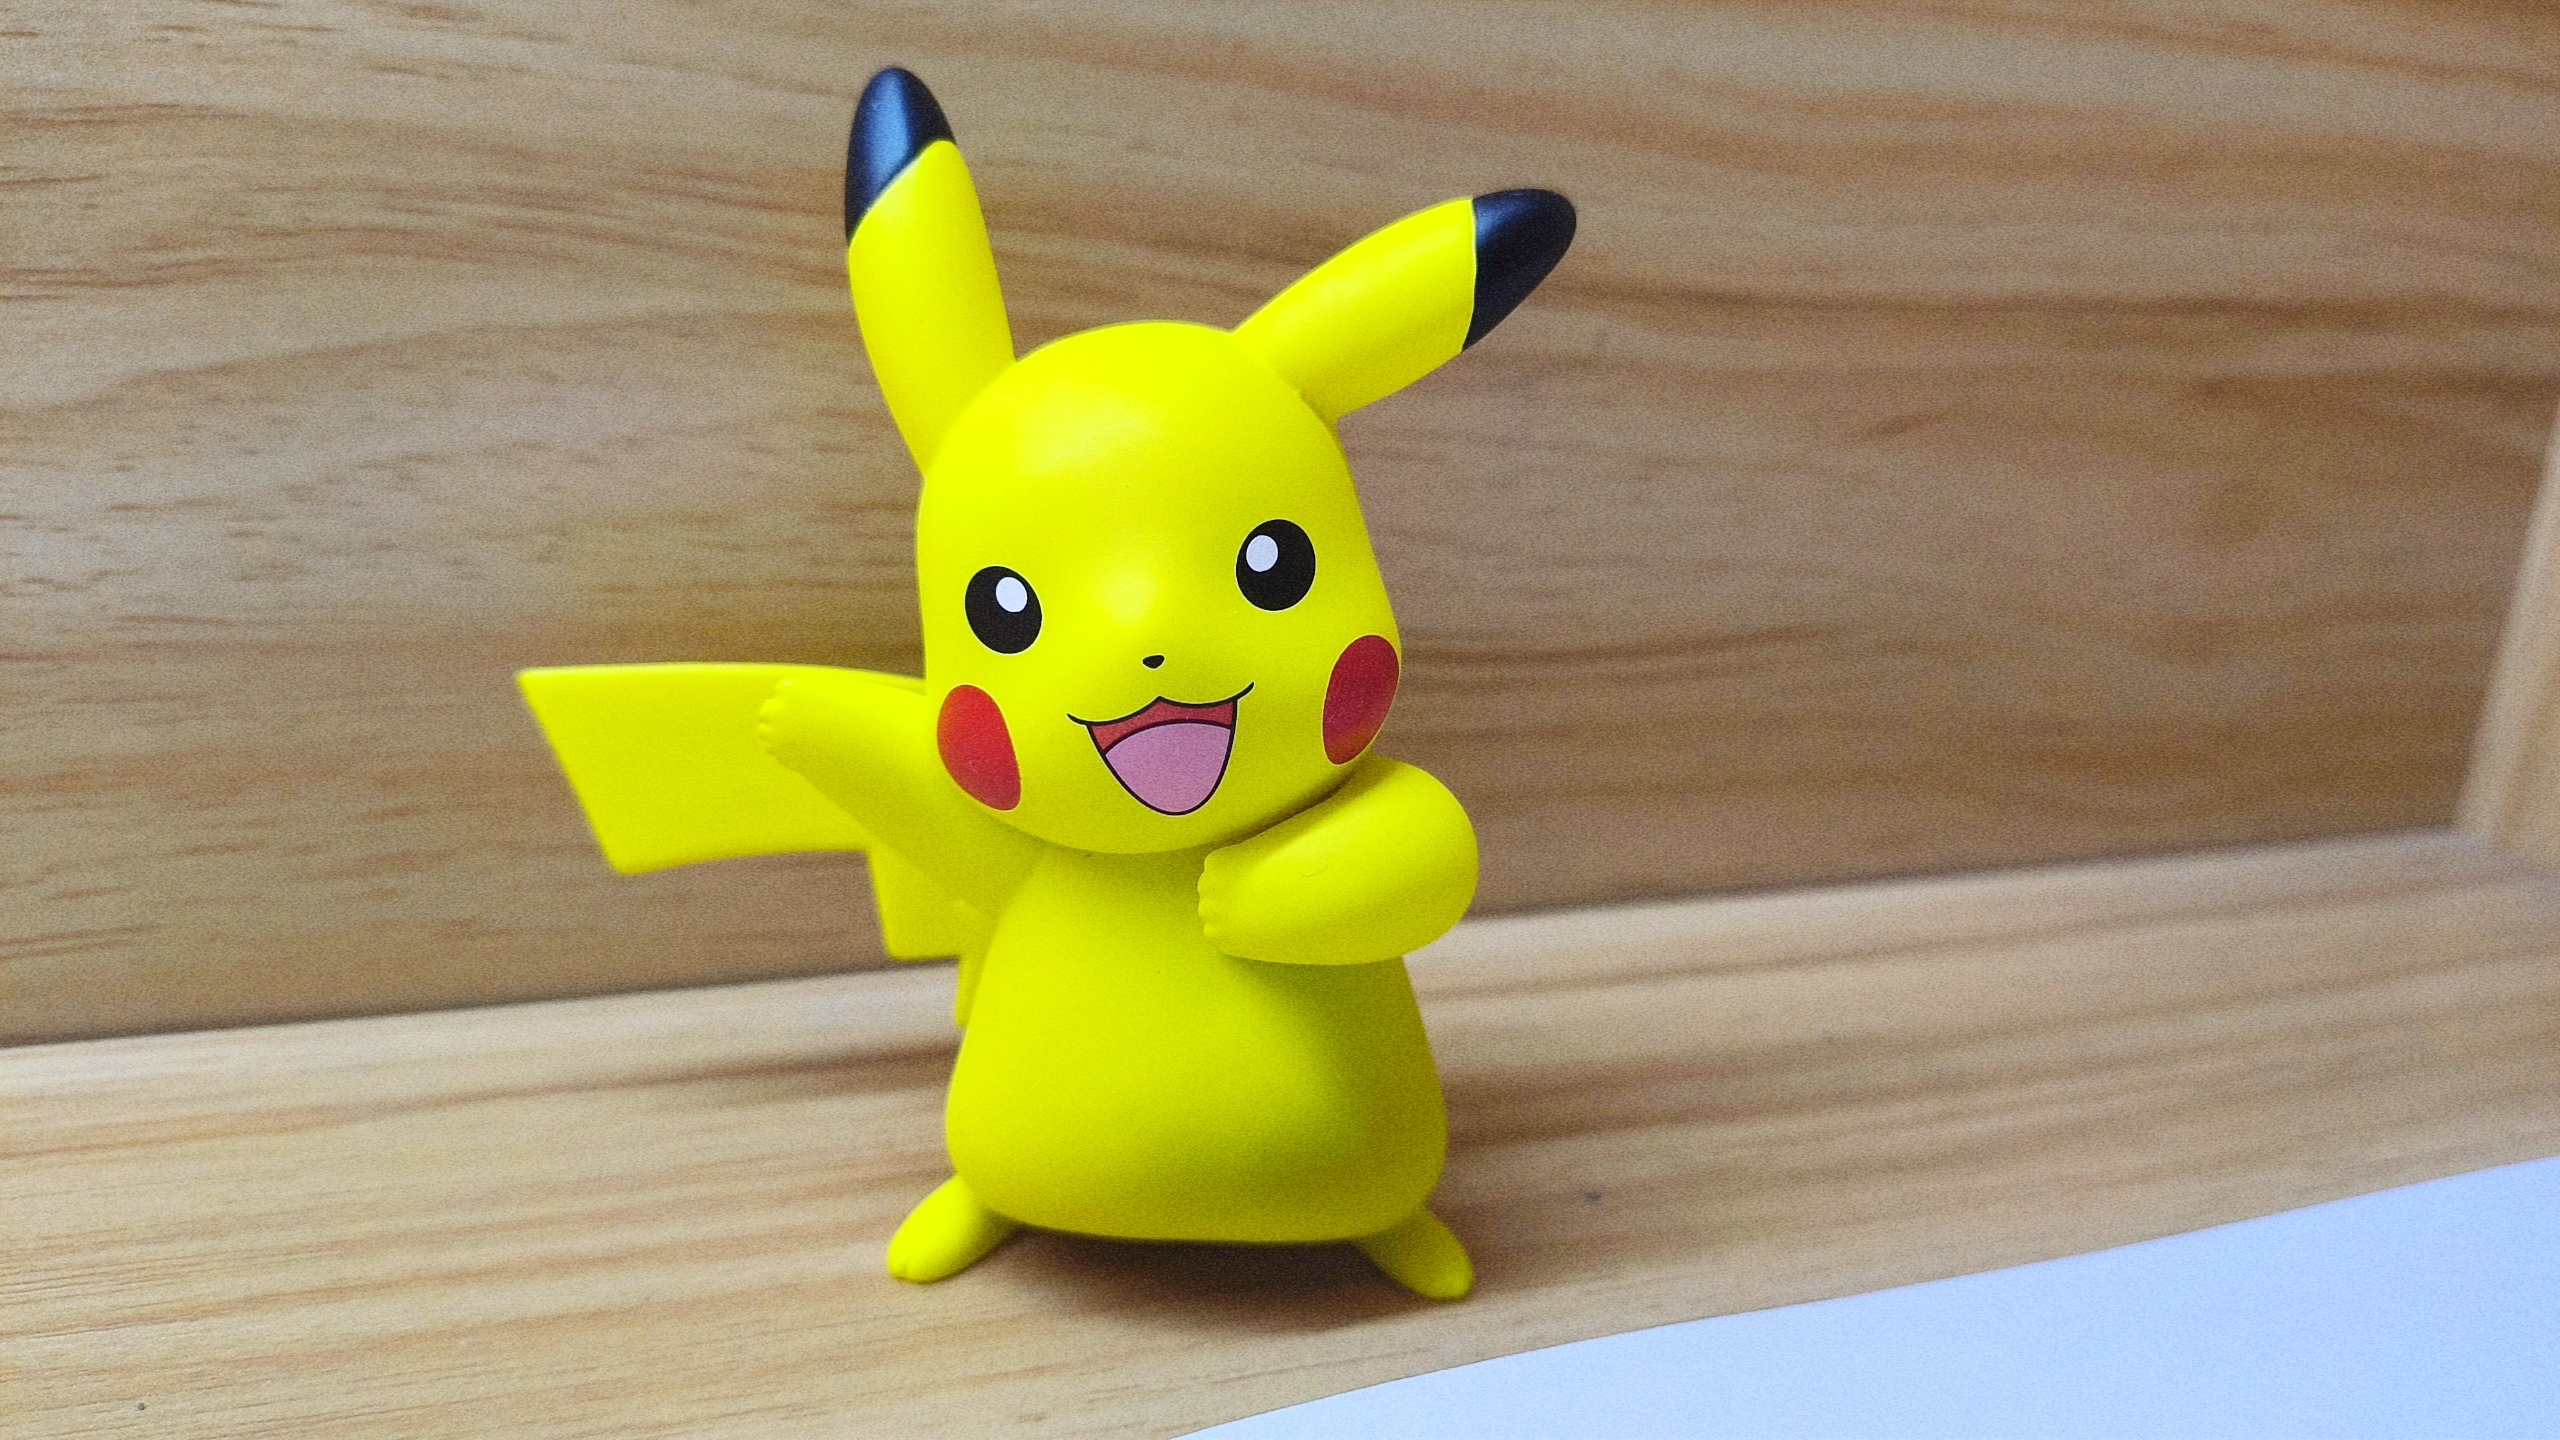
\includegraphics[scale=0.1]{figures/pikachu.jpg}
        \caption{这是图片}
        \label{fig:2}
    \end{figure}
    \subsubsection{表格}
    \begin{table}[!htbp]
        \centering
        \caption{这是表格}
        \begin{tabular}{cccccc}
            \toprule
            序号 & 姓名 & 性别 & 年龄 & 身高/cm & 体重/kg \\
            \midrule
            1 & 张三 & M & 16 & 163 & 50 \\
            2 & 王红 & F & 15 & 159 & 47 \\
            3 & 李二 & M & 17 & 165 & 52 \\
            \bottomrule
        \end{tabular}
        \label{tab:2}
    \end{table}
    \subsection{交叉引用}\label{sec:3}
    \subsubsection{参考文献引用}\label{sec:4}
    首先引用一下大名鼎鼎的香农信息论\cite{shannon1948mathematical},所以哪能少得了图灵\cite{turing2009computing},因为看过《美丽心灵》就还有纳什\cite{nash1996non}。
    \subsubsection{图表引用}
    图片\ref{fig:2}和表格\ref{tab:2}的交叉引用。
    \subsubsection{章节引用}
    章节\ref{sec:3}和章节\ref{sec:4}的交叉引用。
    \subsubsection{公式引用}
    公式\ref{eq:2}的交叉引用。
% ·································································································
\end{ujnbody}